\chapter{Resultados y Análisis}

Tal y como se puede apreciar en el diagrama de flujo de CRISP-ML(Q)\ref{fig:crispml-q-diagram}, la Preparación de los datos es un paso crucial en el desarrollo. Tal es así, que son 4 las tareas definidas en Scrum para ello:
\begin{itemize}
    \item PD-1: normalizar y codificar variables.
    \item PD-2: manejar valores atípicos y nulos.
    \item PD-3: definir proporción de sepación de datos.
    \item PD-4: verificar balanceo de clases.
\end{itemize}

Las dos últimas, PD-3 y PD-4, inferirán de manera capital en la calidad de los resultados; pero las dos primeras son las que harán que el entrenamiento se pueda llevar a cabo o no, las que harán que la programación discurra por unos derroteros u otros, dependiendo del nivel de ``suciedad'' o divergencia que se encuentre en los datos y del nivel de homogeneidad que se demande.

Así pues, se procede a realizar un análisis exploratorio de datos, en aras de conocer amortiguar en la medida de lo posible, todas las dificultades que puedan encontrarse.

\section{Análisis Exploratorio de Datos (EDA)}

El análisis exploratorio de datos constituye un paso esencial en este estudio sobre la generación de música personalizada mediante modelos generativos adversariales (GANs). Se han utilizado tres conjuntos de datos principales: \textbf{FMA (Free Music Archive)}, \textbf{Million Song Dataset} y \textbf{MTG-Jamendo}, los cuales contienen una amplia diversidad de géneros y metadatos relacionados.

\subsection{Distribución de los datos}
Se ha trabajado con un total de \textbf{176,500 pistas de audio}, distribuidas de la siguiente manera:
\begin{itemize}
\item \textbf{FMA Large}: 106,000 pistas, 161 géneros.
\item \textbf{Million Song Dataset}: 25,000 pistas, 15 géneros.
\item \textbf{MTG-Jamendo Dataset}: 50,000 pistas, 190 géneros.
\end{itemize}

Para garantizar la coherencia del conjunto de datos:
\begin{itemize}
\item Se han filtrado archivos corruptos o incompletos.
\item Se ha unificado la estructura de etiquetas de género.
\item Se ha establecido una duración uniforme de \textbf{30 segundos} para cada clip de audio. (Esta duración se podrá ver modificada según sea la experiencia durante el entrenamiento. La duración más conservadora elegible serían 25 segundos, pues están asegurados en todas las muestras de los 3 conjuntos).
\end{itemize}

\subsection{Distribución de géneros}
Los cinco géneros musicales más representados en la base de datos son:
\begin{enumerate}
\item Rock (35,200 pistas)
\item Pop (30,100 pistas)
\item Jazz (22,800 pistas)
\item Hip-Hop (19,500 pistas)
\item Electrónica (17,900 pistas)
\end{enumerate}

Se realizaá un análisis espectral de los archivos de audio mediante \textbf{MFCCs (Mel-Frequency Cepstral Coefficients)} y \textbf{espectrogramas de corto tiempo (STFT)}. Esto permitió visualizar la distribución de frecuencias y la evolución de los patrones tonales en los diferentes géneros.

\section{Evaluación}

Este apartado recoge el procedimiento empleado para evaluar el rendimiento de los modelos generativos propuestos: un autoencoder variacional (VAE) y una arquitectura GAN con generador basado en Transformer. Se han utilizado tanto métricas cuantitativas como cualitativas, adaptadas al dominio musical y al uso de espectrogramas STFT como representación intermedia.

\subsection{Modelos evaluados}

\subsubsection*{Variational Autoencoder (VAE)}

El modelo VAE implementa un esquema encoder-decoder convolucional condicionado por género, que utiliza una función de pérdida compuesta por dos términos:

\[
\mathcal{L} = \underbrace{\|x - \hat{x}\|^2}_{\text{Reconstrucción}} + \beta \cdot \underbrace{D_{\text{KL}}\left(q(z|x) \,||\, \mathcal{N}(0, I)\right)}_{\text{Divergencia KL}}
\]

donde:
\begin{itemize}
    \item $x$ es el espectrograma STFT original.
    \item $\hat{x}$ es el espectrograma reconstruido.
    \item $\beta \in \mathbb{R}$ es un coeficiente dinámico regulado con función sigmoide durante el \textit{warmup}:
\end{itemize}

\[
\beta = \min\left( \frac{\beta_{\max}}{1 + e^{-10 (\text{epoch} / \text{warmup} - 0.5)}}, \beta_{\max} \right)
\]

La divergencia KL se calcula por lote según:

\[
D_{\text{KL}} = -\frac{1}{2} \sum_{i=1}^{d} \left(1 + \log(\sigma_i^2) - \mu_i^2 - \sigma_i^2\right)
\]

donde $\mu$ y $\log\sigma^2$ son los parámetros del espacio latente aprendidos por el encoder.

\subsubsection*{Generative Adversarial Network (GAN + Transformer)}

El modelo GAN consta de dos redes entrenadas en competencia:

\begin{itemize}
    \item \textbf{Generador} $G(z, y)$: transforma un vector de ruido $z \sim \mathcal{N}(0, I)$ y un embedding de género $y$ en un espectrograma STFT sintético.
    \item \textbf{Discriminador} $D(x, y)$: predice si un espectrograma dado $x$ es real o generado, condicionado también por el género.
\end{itemize}

Durante la fase principal del entrenamiento, ambos modelos se optimizan mediante una función de pérdida adversarial binaria:

\[
\mathcal{L}_D = -\frac{1}{2} \left[ \log D(x_{\text{real}}, y) + \log (1 - D(G(z, y), y)) \right]
\]
\[
\mathcal{L}_G = -\log D(G(z, y), y)
\]

\medskip

\noindent Durante las primeras épocas se aplica un \textbf{preentrenamiento} por separado a cada red:

\begin{itemize}
    \item \textbf{Preentrenamiento del generador}: consiste en una reconstrucción supervisada, forzando al generador a aproximarse a un espectrograma real a través de un vector de ruido inicializado aleatoriamente. Se emplea pérdida MSE:
    
    \[
    \mathcal{L}^{\text{pretrain}}_G = \| G(z, y) - x_{\text{real}} \|^2
    \]

    donde $x_{\text{real}}$ es un espectrograma recortado a una duración fija y normalizado.
    
    \item \textbf{Preentrenamiento del discriminador}: se entrena para reconocer espectrogramas reales como positivos mediante clasificación binaria con entropía cruzada:

    \[
    \mathcal{L}^{\text{pretrain}}_D = -\left[ y \cdot \log D(x, y) + (1 - y) \cdot \log(1 - D(x, y)) \right]
    \]

    En esta etapa sólo se utilizan muestras reales, por lo que $y = 1$ en todos los casos. Es decir, se le entrena a clasificar correctamente datos auténticos como verdaderos.
\end{itemize}

Este procedimiento busca estabilizar la formación de las dos redes antes de introducir la dinámica adversarial completa.


\subsubsection*{Estrategia de validación}

Para todos los modelos evaluados, se ha aplicado una estrategia de validación constante con partición aleatoria del conjunto de datos:

\[
\texttt{val\_split = 0.2}
\]

Esto implica que el 80\% del dataset se emplea para entrenamiento y el 20\% restante para validación. La división se realiza una sola vez al inicio del entrenamiento, utilizando la función \texttt{random\_split()} sobre el conjunto completo.

La validación se ejecuta al final de cada época, registrando las mismas métricas que en entrenamiento, pero sin actualización de pesos. Esta estrategia permite monitorizar el sobreajuste y la generalización del modelo sobre datos no vistos durante el aprendizaje.

\subsection{Métricas de evaluación}

\subsubsection*{Métricas cuantitativas}

\begin{itemize}
    \item \textbf{Pérdida de reconstrucción (VAE)}: error cuadrático medio entre espectrogramas reales y reconstruidos.
    \item \textbf{Divergencia KL (VAE)}: regularización del espacio latente respecto a una distribución normal.
    \item \textbf{Pérdida adversarial (GAN)}: pérdida binaria cruzada tanto para el generador como para el discriminador.
    \item \textbf{Consistencia temporal (opcional)}: medida no entrenada que evalúa la diferencia espectral entre marcos adyacentes.
\end{itemize}

\subsubsection*{Métricas cualitativas}

\begin{itemize}
    \item \textbf{Inspección visual}: comparación entre espectrogramas reales y generados por el modelo.
    \item \textbf{Evaluación subjetiva}: análisis humano de naturalidad, coherencia musical y progresión temporal.
\end{itemize}

\subsection{Registro y evolución de pérdidas}

Durante el entrenamiento se han registrado, por batch y por época:

\begin{itemize}
    \item Para VAE: \texttt{total\_loss}, \texttt{recon\_loss}, \texttt{kl\_divergence}, \texttt{beta}.
    \item Para GAN:
        \begin{itemize}
            \item En preentrenamiento: \texttt{pretrain\_g\_loss}, \texttt{pretrain\_d\_loss}.
            \item En fase adversarial: \texttt{g\_loss}, \texttt{d\_loss}.
        \end{itemize}
\end{itemize}

Los valores son utilizados tanto para análisis posterior como para implementar estrategias de parada temprana (\textit{early stopping}) y selección de checkpoints.



\subsection{Modelos evaluados}

En este apartado se describen las arquitecturas reales desarrolladas para la generación de música basada en espectrogramas STFT. Se detallan las decisiones estructurales, el flujo de datos y las funciones de pérdida utilizadas en cada caso, basándose directamente en el código fuente implementado en PyTorch Lightning y parametrizado por variables del entorno (.env).

\subsubsection*{5.3.1 VAE convolucional con decoder LSTM}

El modelo VAE implementado combina un encoder convolucional con un decoder que incorpora una capa LSTM, con condicionamiento explícito por género en ambas etapas.

\paragraph{Encoder:} el encoder aplica tres bloques \texttt{Conv2d + BatchNorm + ReLU + MaxPool2d} sobre la entrada, que es un espectrograma de dimensiones $(1, 128, T)$ concatenado con un embedding de género expandido a la misma resolución espacial. Tras la convolución, se aplana el resultado y se proyecta a dos vectores: $\mu \in \mathbb{R}^{d}$ y $\log\sigma^2 \in \mathbb{R}^{d}$ mediante capas lineales:

\[
z \sim \mathcal{N}(\mu, \sigma^2) \quad \text{mediante reparametrización:} \quad z = \mu + \sigma \cdot \epsilon
\]

\paragraph{Decoder:} el decoder concatena $z$ con el embedding de género, lo proyecta a un tensor de tamaño $C \times H \times W$ mediante una capa lineal, y lo rearma como tensor convolucional. Posteriormente:

\begin{itemize}
    \item Se aplica una LSTM sobre la dimensión temporal (transformando $B \times C \times H \times W$ en secuencias de $W$ pasos).
    \item Se reconstruye el espectrograma mediante tres capas \texttt{ConvTranspose2d}.
    \item Se recorta o rellena a $T$ pasos temporales y se normaliza en decibelios.
\end{itemize}

\paragraph{Pérdida:} se emplea una pérdida compuesta:

\[
\mathcal{L}_{\text{VAE}} = \underbrace{\|x - \hat{x}\|^2}_{\text{Reconstrucción}} + \beta \cdot \underbrace{D_{\text{KL}}(\mathcal{N}(\mu, \sigma^2) \parallel \mathcal{N}(0, I))}_{\text{Regularización latente}}
\]

El parámetro $\beta$ se incrementa progresivamente mediante una función sigmoide durante el \textit{warm-up}, parametrizado por \texttt{BETA\_WARMUP\_EPOCHS} y \texttt{BETA\_MAX}.

\paragraph{Monitorización adicional:} el modelo almacena la media y desviación típica de entrada $x$, registra métricas por batch y época, actualizando también los límites de decibelios por género en un archivo JSON persistente, que se usará como límites de decibelios en la generación.

\vspace{1em}

\subsubsection*{5.3.2 GAN con generador TransformerEncoder}

La arquitectura GAN consta de dos componentes diferenciados: un generador con Transformer y un discriminador convolucional.

\paragraph{Generador:}
\begin{itemize}
    \item La entrada es un vector de ruido $z \in \mathbb{R}^{d}$ concatenado con el embedding del género.
    \item Se proyecta a una secuencia de $T$ tokens de dimensión $d_{\text{model}}$ mediante una capa lineal.
    \item Se aplica un bloque \texttt{TransformerEncoder} con $L$ capas, $h$ cabezas y \texttt{dim\_feedforward}, definidos en \texttt{.env}.
    \item La salida se transforma en un espectrograma de dimensiones $(1, 128, T)$ mediante dos capas \texttt{Conv1d} y activación \texttt{Tanh}.
\end{itemize}

\paragraph{Discriminador:}
\begin{itemize}
    \item Concatenación del espectrograma $(1, 128, T)$ con el embedding de género expandido espacialmente.
    \item Tres bloques convolucionales seguidos de \texttt{BatchNorm}, \texttt{ReLU} y \texttt{MaxPool2d}.
    \item Aplanado y paso por una capa lineal que produce un único logit: probabilidad de real/falso.
\end{itemize}

\paragraph{Preentrenamiento:} se realizan dos fases iniciales:

\begin{align*}
\text{Generador:} \quad & \mathcal{L}^{\text{pretrain}}_G = \| G(z, y) - x_{\text{real}} \|^2 \\
\text{Discriminador:} \quad & \mathcal{L}^{\text{pretrain}}_D = -\log D(x_{\text{real}}, y)
\end{align*}

\paragraph{Fase adversarial:} durante el entrenamiento completo, se utilizan pérdidas de tipo BCE:

\begin{align*}
\mathcal{L}_D &= -\frac{1}{2} \left[ \log D(x_{\text{real}}, y) + \log(1 - D(G(z, y), y)) \right] \\
\mathcal{L}_G &= -\log D(G(z, y), y)
\end{align*}

\paragraph{Estrategia de entrenamiento:} se entrena alternativamente el discriminador y el generador, con optimización manual mediante \texttt{self.manual\_backward()} y uso de dos optimizadores separados tipo Adam.

\vspace{1em}

\subsubsection*{Comparativa}

\begin{itemize}
    \item \textbf{VAE}: destaca en reconstrucción precisa y codificación interpretativa. Su decoder con LSTM permite una mayor coherencia temporal local.
    \item \textbf{GAN}: genera muestras completamente nuevas desde ruido, con mayor capacidad creativa. El uso del Transformer permite capturar dependencias de largo alcance en el tiempo.
\end{itemize}

Ambos modelos están condicionados por género, parametrizados mediante `.env` y adaptados para espectrogramas de tamaño $(128, T)$ derivados de audio a 44.1 kHz.

\subsection{Resultados}

El entrenamiento se lleva a cabo con fragmentos de audio que han de cumplir:
\begin{itemize}
    \item que sean accesibles (que exista el fichero declarado en los metadatos del dataset).
    \item al menos \textbf{30 segundos de duración}.
    \item que no estén corruptos.
    \item \emph{\# sample rate} de al menos \textbf{44100 Hz} (si es mayor, se efectúa un \emph{\# downsampling}).
\end{itemize}

Una vez hecho esto, para asegurar que no existan problemas al final de la pista (algunas pistas fallaban en el tratamiento final o contenían sonidos extraños), se hace un corte a \textbf{25 segundos}.

Tasadas las piezas en 25 segundos, se toman muestras de audio de 5 en 5 segundos, que será la cantidad de sonido por pista que procesen de una vez.

\begin{figure}[H]
    \centering
    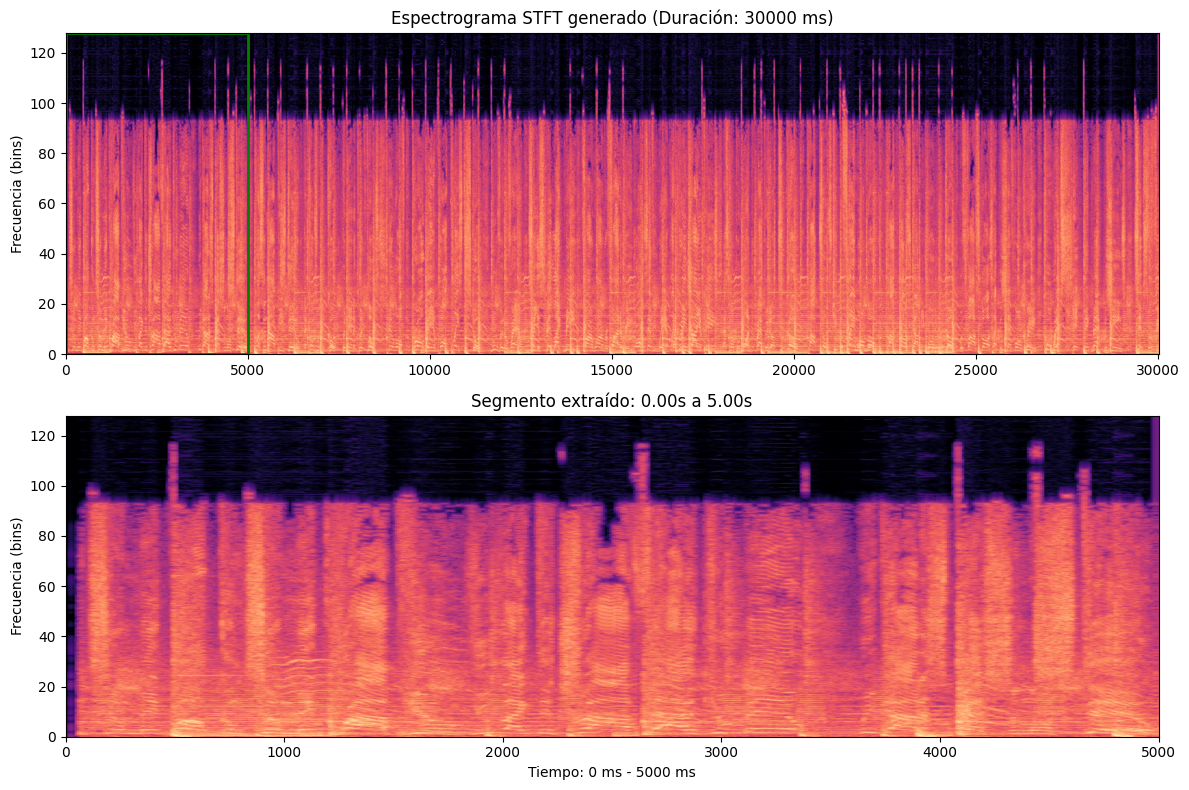
\includegraphics[width=0.6\textwidth]{images/spect_window_1.png}
    \caption{Primera ventana de espectrograma. De 0 a 5 segundos}
\end{figure}
\begin{figure}[H]
\centering
\resizebox{0.7\textwidth}{!}{
    \begin{minipage}{\textwidth}
    \centering
    \begin{subfigure}[t]{0.48\textwidth}
        \centering
        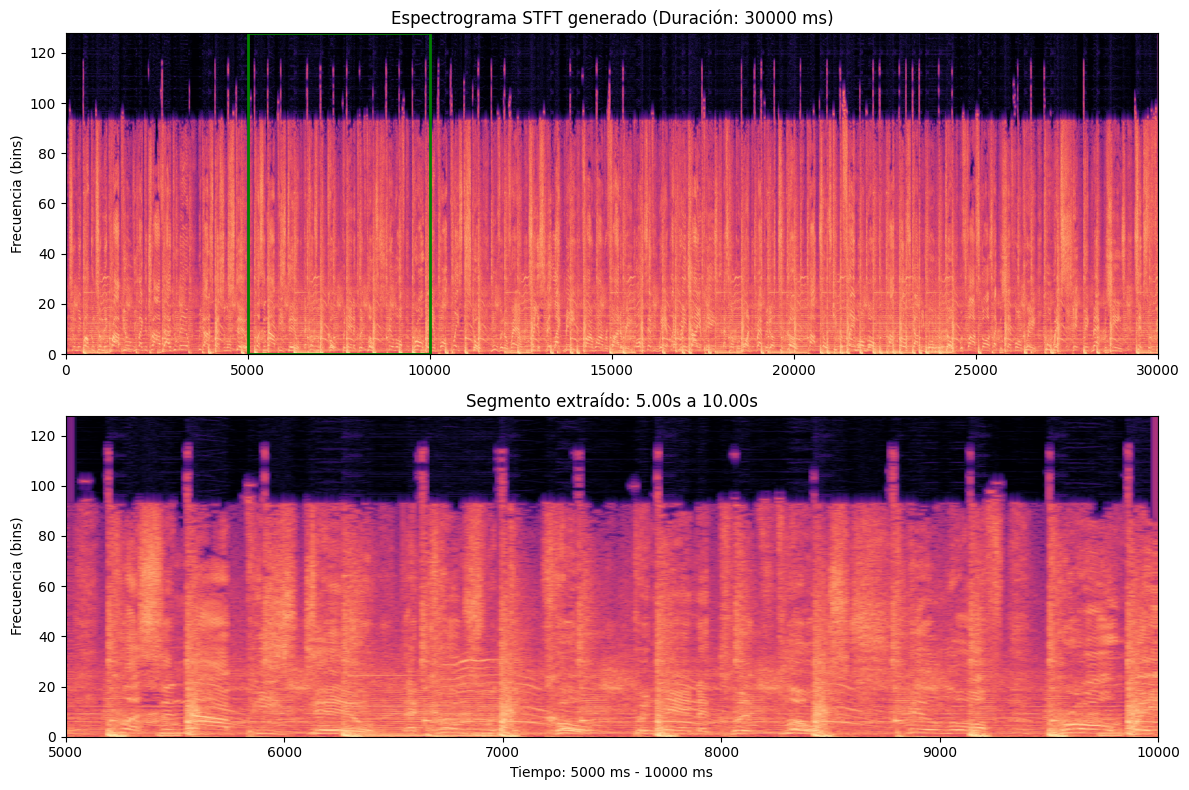
\includegraphics[width=\textwidth]{images/spect_window_2.png}
        \caption{Segunda ventana de espectrograma. De 5 a 10 segundos}
    \end{subfigure}
    \hfill
    \begin{subfigure}[t]{0.48\textwidth}
        \centering
        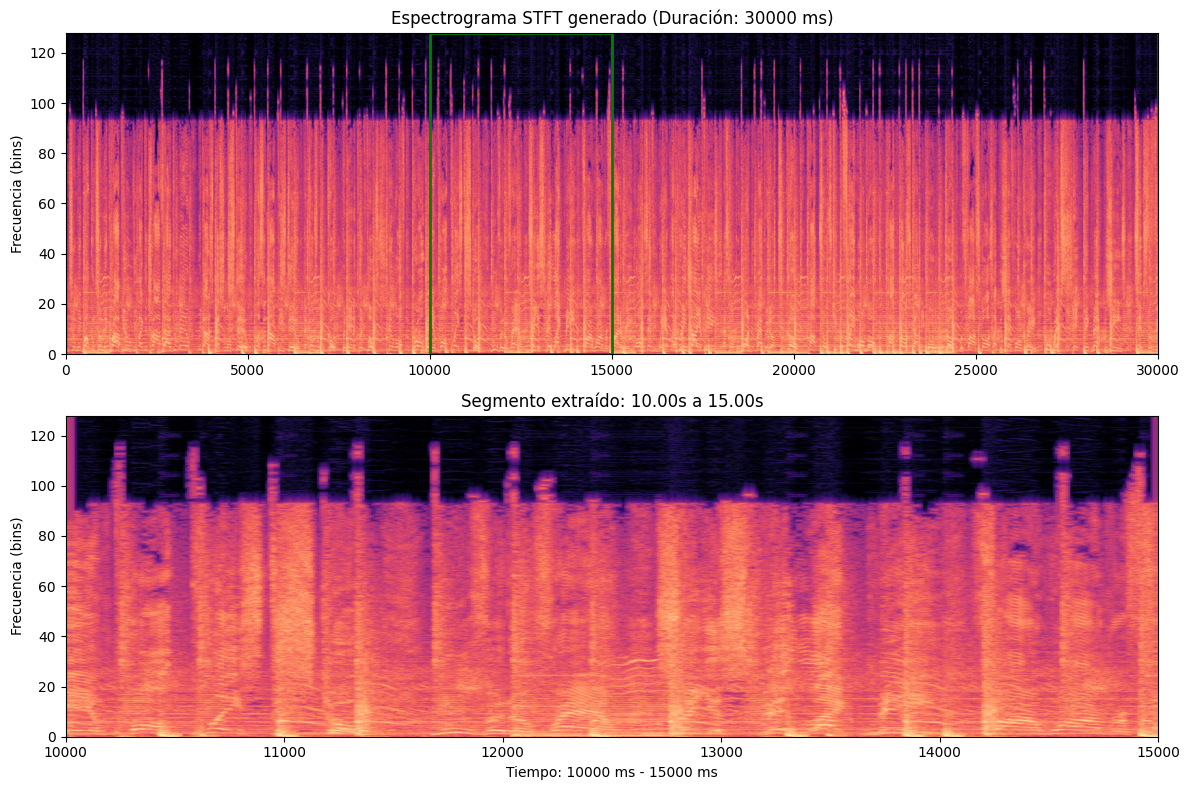
\includegraphics[width=\textwidth]{images/spect_window_3.png}
        \caption{Tercera ventana de espectrograma. De 10 a 15 segundos}
    \end{subfigure}
    \end{minipage}
}
\caption{Segunda y tercera ventana de espectrograma.}
\label{fig:diseno-paneles}
\end{figure}
\begin{figure}[H]
    \centering
    \resizebox{0.7\textwidth}{!}{
        \begin{minipage}{\textwidth}
        \centering
        \begin{subfigure}[t]{0.48\textwidth}
            \centering
            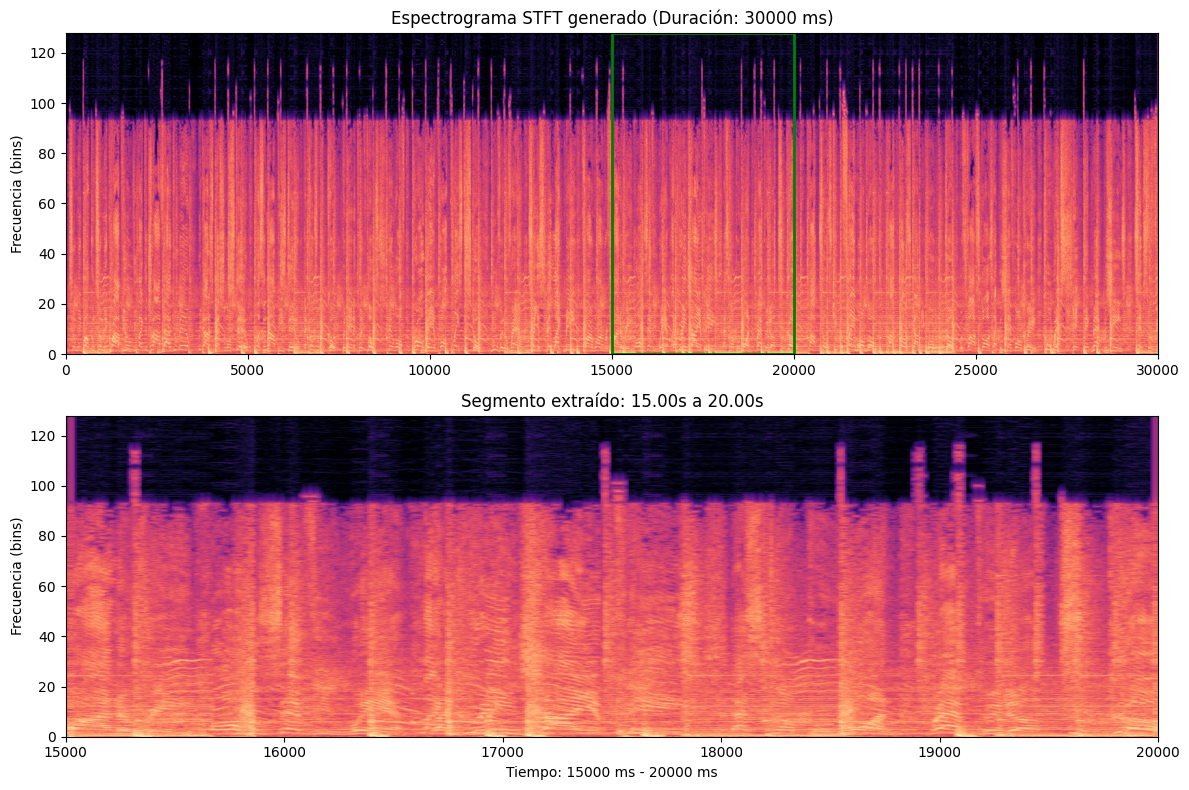
\includegraphics[width=\textwidth]{images/spect_window_4.png}
            \caption{Cuarta ventana de espectrograma. De 15 a 20 segundos}
        \end{subfigure}
        \hfill
        \begin{subfigure}[t]{0.48\textwidth}
            \centering
            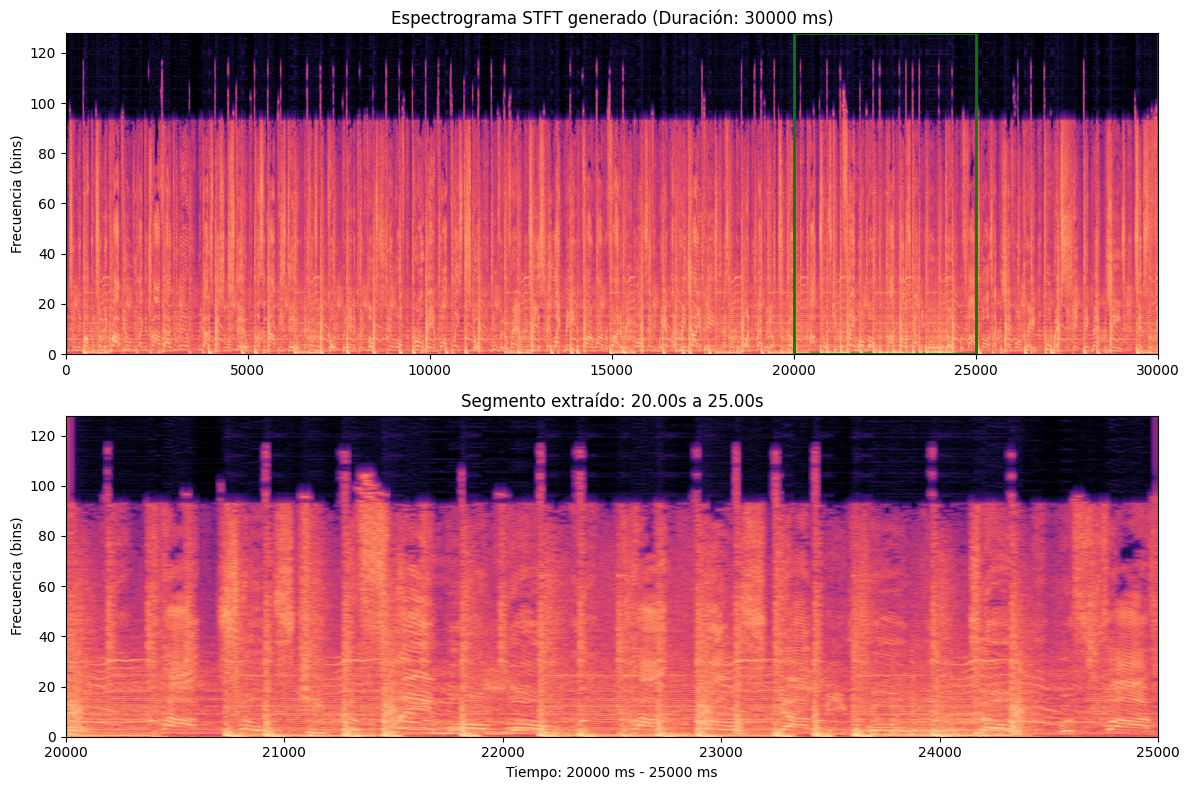
\includegraphics[width=\textwidth]{images/spect_window_5.png}
            \caption{Quinta ventana de espectrograma. De 20 a 25 segundos}
        \end{subfigure}
        \end{minipage}
    }
    \caption{Cuarta y quinta ventana de espectrograma.}
    \label{fig:diseno-paneles}
    \end{figure}


\subsubsection{Conditional VAE. Otro método de orientación al error}

\subsection*{Hiperparámetros utilizados}

Los siguientes hiperparámetros han sido definidos en el archivo \texttt{.env} para configurar el preprocesamiento de datos, el entrenamiento y la arquitectura de los modelos.

\begin{itemize}
  \item \textbf{Parámetros generales:}
  \begin{itemize}
    \item \textbf{SAMPLE\_RATE}: 44100 \emph{\# Frecuencia de muestreo del audio (Hz)}.
    \item \textbf{N\_FFT}: 2048 \emph{\# Número de puntos de FFT para la STFT}.
    \item \textbf{HOP\_LENGTH}: 440 \emph{\# Desplazamiento entre ventanas en la STFT}.
    \item \textbf{TOTAL\_DURATION}: 25 \emph{\# Duración total de los archivos de audio (segundos)}.
    \item \textbf{SEGMENT\_DURATION}: 5 \emph{\# Duración de cada segmento de entrada al modelo (segundos)}.
    \item \textbf{NUM\_MELS}: 128 \emph{\# Número de bandas mel o bins espectrales en el espectrograma}.
    \item \textbf{NUM\_GENRES}: 5 \emph{\# Número de géneros musicales distintos}.
    \item \textbf{KIND\_OF\_SPECTROGRAM}: STFT \emph{\# Tipo de espectrograma utilizado, pudiendo ser MEL}.
  \end{itemize}

  \item \textbf{Entrenamiento:}
  \begin{itemize}
    \item \textbf{TRAIN\_BATCH\_SIZE}: 2 \emph{\# Tamaño de batch durante el entrenamiento}.
    \item \textbf{TRAIN\_EPOCHS}: 30 \emph{\# Número total de épocas de entrenamiento}.
    \item \textbf{LIMIT\_FILES}: 1000 \emph{\# Número máximo de archivos usados (modo prueba)}.
  \end{itemize}

  \item \textbf{VAE:}
  \begin{itemize}
    \item \textbf{LATENT\_DIM}: 1024 \emph{\# Dimensión del espacio latente $z$}.
    \item \textbf{BETA\_MAX}: 4.0 \emph{\# Valor máximo del coeficiente $\beta$ en la pérdida del VAE}.
    \item \textbf{BETA\_WARMUP\_EPOCHS}: 20 \emph{\# Número de épocas de \textit{warm-up} progresivo para $\beta$}.
  \end{itemize}

\end{itemize}

\subsubsection*{Optimizador utilizado en el VAE}

El modelo VAE se entrena utilizando el optimizador \textbf{Adam}, complementado con un \textbf{\emph{scheduler} de reducción por meseta} para ajustar dinámicamente la tasa de aprendizaje en función del rendimiento del modelo en validación.

\begin{itemize}
    \item \textbf{Optimizador:} \texttt{torch.optim.Adam}
    \item \textbf{Tasa de aprendizaje} (\texttt{lr}): \textit{1e-3}
    \begin{itemize}
        \item Este valor es adecuado para redes convolucionales profundas con funciones de pérdida suavizadas como MSE + KL.
        \item Un valor mayor podría producir oscilaciones en la KL o en la salida del decoder, mientras que un valor menor ralentizaría la convergencia.
    \end{itemize}

    \item \textbf{Política de ajuste (scheduler):} \texttt{torch.optim.lr\_scheduler.ReduceLROnPlateau}
    \item \textbf{Criterio de reducción:}
    \begin{itemize}
        \item \textbf{Monitor}: \texttt{val\_loss} — se observa la pérdida en validación.
        \item \textbf{Modo}: \texttt{"min"} — se reduce la tasa de aprendizaje cuando la pérdida deja de disminuir.
        \item \textbf{Paciencia}: \textit{5} — número de épocas consecutivas sin mejora antes de activar la reducción.
        \item \textbf{Factor}: \textit{0.5} — la tasa de aprendizaje se multiplica por este factor (reducción al 50\%).
        \item \textbf{Frecuencia}: \textit{1} — el control se realiza al final de cada época.
    \end{itemize}

    \item \textbf{Justificación:}
    \begin{itemize}
        \item El uso del scheduler evita que el modelo quede estancado si no encuentra una dirección de mejora.
        \item La combinación de Adam con reducción adaptativa mejora la estabilidad durante el balance entre la pérdida de reconstrucción y la divergencia KL.
    \end{itemize}
\end{itemize}

\noindent Esta configuración permite un entrenamiento eficiente, reduciendo automáticamente la tasa de aprendizaje cuando el modelo ha dejado de mejorar, sin necesidad de una programación manual de la misma.


\subsubsection{GAN \emph{from scratch}}

De manera análoga al modelo anterior, los hiperparámetros configurados en el fichero \texttt{.env} son:

\begin{itemize}
  \item \textbf{Parámetros generales:}
  \begin{itemize}
    \item \textbf{SAMPLE\_RATE}: 44100 \emph{\# Frecuencia de muestreo del audio (Hz)}.
    \item \textbf{N\_FFT}: 2048 \emph{\# Número de puntos de FFT para la STFT}.
    \item \textbf{HOP\_LENGTH}: 440 \emph{\# Desplazamiento entre ventanas en la STFT}.
    \item \textbf{TOTAL\_DURATION}: 25 \emph{\# Duración total de los archivos de audio (segundos)}.
    \item \textbf{SEGMENT\_DURATION}: 5 \emph{\# Duración de cada segmento de entrada al modelo (segundos)}.
    \item \textbf{NUM\_MELS}: 128 \emph{\# Número de bandas mel o bins espectrales en el espectrograma}.
    \item \textbf{NUM\_GENRES}: 5 \emph{\# Número de géneros musicales distintos}.
    \item \textbf{KIND\_OF\_SPECTROGRAM}: STFT \emph{\# Tipo de espectrograma utilizado, pudiendo ser MEL}.
  \end{itemize}

  \item \textbf{Entrenamiento:}
  \begin{itemize}
    \item \textbf{TRAIN\_BATCH\_SIZE}: 4 \emph{\# Tamaño de batch durante el entrenamiento}.
    \item \textbf{TRAIN\_EPOCHS}: 50 \emph{\# Número total de épocas de entrenamiento}.
    \item \textbf{LIMIT\_FILES}: 1000 \emph{\# Número máximo de archivos usados (modo prueba)}.
  \end{itemize}

  \item \textbf{GAN + Transformer:}
  \begin{itemize}
    \item \textbf{GENRE\_EMBED\_DIM}: 32 \emph{\# Dimensión del embedding de género}.
    \item \textbf{GEN\_MODEL\_DIM}: 128 \emph{\# Dimensión interna del generador Transformer}.
    \item \textbf{GEN\_NUM\_LAYERS}: 2 \emph{\# Número de capas en el \texttt{TransformerEncoder}}.
    \item \textbf{GEN\_NUM\_HEADS}: 4 \emph{\# Número de cabezas de atención en cada capa del Transformer}.
    \item \textbf{GAN\_PRETRAIN\_EPOCHS\_D}: 5 \emph{\# Épocas de preentrenamiento del discriminador}.
    \item \textbf{GAN\_PRETRAIN\_EPOCHS\_G}: 5 \emph{\# Épocas de preentrenamiento del generador}.
  \end{itemize}
\end{itemize}

El entrenamiento de la arquitectura GAN se realiza con dos optimizadores separados, uno para el generador y otro para el discriminador. Ambos utilizan el algoritmo \textbf{Adam}, una técnica de optimización basada en gradientes adaptativos ampliamente utilizada en el entrenamiento de redes profundas.

\begin{itemize}
    \item \textbf{Optimizador:} \texttt{torch.optim.Adam}
    \item \textbf{Tasa de aprendizaje} (\texttt{lr}): \textit{2e-4}
    \begin{itemize}
        \item Este valor es típico en arquitecturas GAN, ya que una tasa más alta puede provocar inestabilidad, y una demasiado baja puede ralentizar la convergencia.
    \end{itemize}
    \item \textbf{Parámetros \texttt{betas}}: $(0.5,\ 0.999)$
    \begin{itemize}
        \item $\beta_1 = 0.5$: controla el promedio móvil del primer momento (media de gradientes).
        \item $\beta_2 = 0.999$: controla el segundo momento (varianza de gradientes).
        \item El valor reducido de $\beta_1$ con respecto al valor por defecto (0.9) se emplea comúnmente en GANs para evitar oscilaciones rápidas e inestabilidad en el entrenamiento adversarial.
    \end{itemize}
    \item \textbf{Separación de optimizadores:}
    \begin{itemize}
        \item Se instancian dos optimizadores distintos:
        \[
        \text{opt\_g} = \text{Adam}(G.\text{parameters()}, \text{lr}, \text{betas})
        \qquad
        \text{opt\_d} = \text{Adam}(D.\text{parameters()}, \text{lr}, \text{betas})
        \]
        \item Esto permite actualizar el generador y el discriminador de manera independiente, alternando sus pasos en cada iteración según la lógica de entrenamiento definida manualmente con \texttt{self.manual\_backward()}.
    \end{itemize}
\end{itemize}

\noindent Esta configuración se ajusta a las recomendaciones clásicas de \textit{Deep Convolutional GANs (DCGAN)} y proporciona una base estable para el entrenamiento adversarial sobre espectrogramas condicionados por género.

